\documentclass[simplex.tex]{subfiles}
% NO NEED TO INPUT PREAMBLES HERE
% packages are inherited; you can compile this on its own

\onlyinsubfile{
\title{NeuroData SIMPLEX Report: Subfile}
}

\begin{document}
\onlyinsubfile{
\maketitle
\thispagestyle{empty}

The following report documents the progress made by the labs of Randal~Burns and Joshua~T.~Vogelstein at Johns Hopkins University towards goals set by the DARPA SIMPLEX grant.

%%%% Table of Contents
\tableofcontents

%%%% Publications
\bibliographystyle{IEEEtran}
\begin{spacing}{0.5}
\section*{Publications, Presentations, and Talks}
%\vspace{-20pt}
\nocite{*}
{\footnotesize	\bibliography{simplex}}
\end{spacing}
%%%% End Publications
}


\subsection{FlashX}

Sparse matrix multiplication in FlashX uses its own format (SCSR) for
sparse matrices to improve performance. We investigated the overhead of
using customized format to thoroughly evaluate the performance of sparse
matrix multiplication in FlashX. Thus, it is essential to accelerate the
format conversion from a standard format such as CSR to our customized
format SCSR. Figure \ref{fig:flashx1}, below, shows the benefit of using
the SCSR format including the overhead of format conversion. When an
application requires more than 4 SpMVs, converting the format of a
sparse matrix improves the performance of the application. Thus,
majority of the applications benefit from the format conversion.

\begin{figure}[h!]
\begin{cframed}
\centering
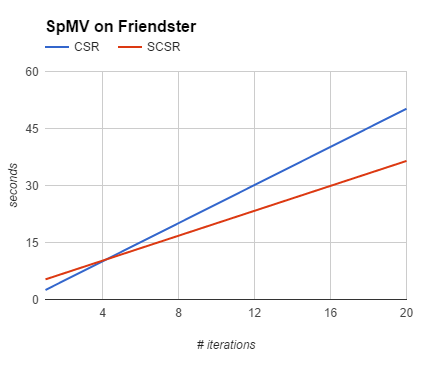
\includegraphics[width=0.45\textwidth]{./figs/SpMV-friendster.png}
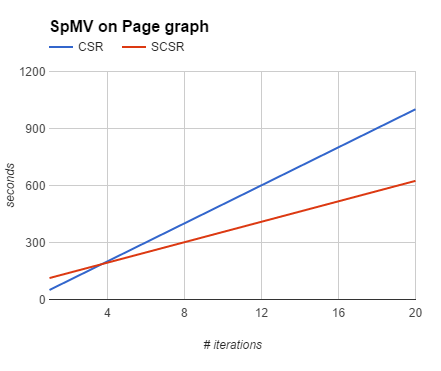
\includegraphics[width=0.45\textwidth]{./figs/SpMV-pagegraph.png}
\caption{
Benefits of using SCSR.
}
\label{fig:flashx1}
\end{cframed}
\end{figure}

The performance ratio of the in-memory and semi-external memory sparse
matrix multiplication in FlashX is affected by multiple factors. Shown
in Figure \ref{fig:flashx2}, we demonstrate some of the factors with SBM
graphs with the same number of vertices and edges. We vary the number of
clusters and the number of edges inside clusters. We measure the
performance of SpMV on both clustered and un-clustered graphs. When
vertices are ordered based on the cluster structure, more clusters and
more edges inside clusters increase CPU cache hits, which leads to less
computation overhead and larger performance gap between in-memory and
semi-external memory executions. However, if vertices are ordered
randomly, these two factors have less obvious impact on performance.

\begin{figure}[h!]
\begin{cframed}
\centering
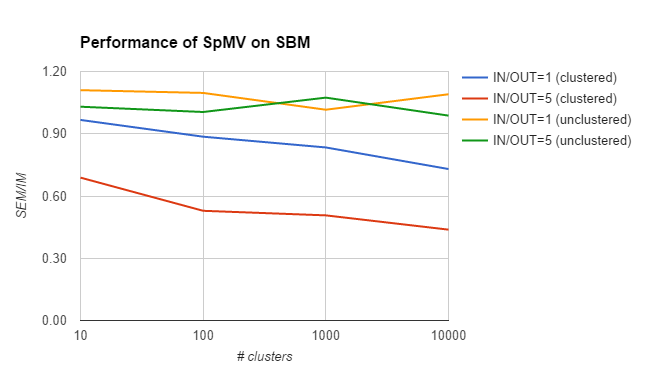
\includegraphics[width=0.75\textwidth]{./figs/SpMV-sbm.png}
\caption{
Benefits of using SCSR.
}
\label{fig:flashx2}
\end{cframed}
\end{figure}

We implement Daniel Lee’s NMF algorithm with our semi-external memory
sparse matrix multiplication (denoted as SEM-NMF) and evaluate its
performance by comparing it with a high-performance NMF implementation
SmallK on billion-scale graphs. The dense matrices for NMF can be as
large as the sparse matrix. As such, we split the dense matrix
vertically so that each of the vertical partitions can fit in memory. We
also evaluate the effect of the memory size on the performance of
SEM-NMF by varying the number of columns in memory from the dense
matrices. In the experiment, we factorize each of the graphs
into two $n \times 16$ non-negative dense matrices.


We significantly improve the performance of SEM-NMF by keeping more
columns of the input dense matrix in memory (Figure \ref{fig:nmf}). The
performance improvement is more significant when the number of columns
that fit in memory is small. When we keep eight columns of the input
dense matrix in memory, SEM-NMF achieves over 60\% of the performance of
its in-memory execution.


SEM-NMF significantly outperforms SmallK and other NMF implementations
in the literature. SmallK is the closest competitor. We run the same NMF
algorithm in SmallK and SEM-NMF outperforms SmallK by a large factor on
all graphs (Figure~\ref{fig:nmf}). There are many MapReduce
implementations in the literature. They run on sparse matrices with tens
of millions of non-zero entries but generally take one or two orders of
magnitude more time than our SEM-NMF on the sparse matrices with
billions of non-zero entries.


\begin{figure}[h!]
\begin{cframed}
\centering
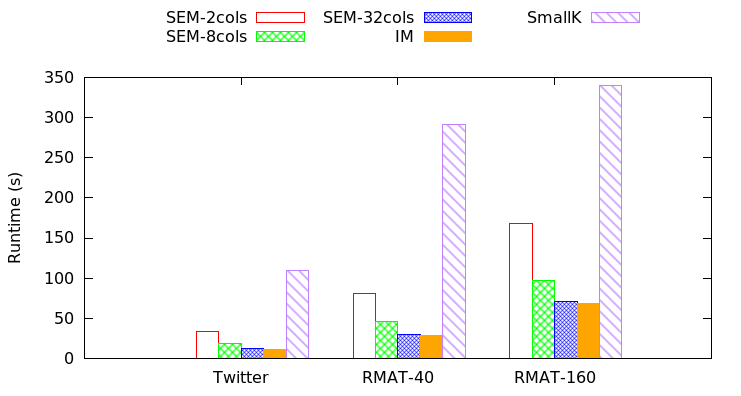
\includegraphics[width=0.5\textwidth]{./figs/nmf.png}
\caption{
Performance improvements of SEM-NMF.
}
\label{fig:nmf}
\end{cframed}
\end{figure}

\end{document}
